\subsection{Variance reduction}
\subsubsection{Cell-based biasing}
\label{sec:vr:cell}

Cell-based weight window can be generated with the following arguments:

\lstinputlisting[language=bash,numbers=none,backgroundcolor=\color{yellow!20},frame=tb]{UserGuide/cell-biasing.sh}



  The purpose of the variance reduction is to change the weight in the cell by the following equation 
  \begin{equation}
    \label{weigthEqn}
    w_{mod}= \textrm{scaleFactor} \times \frac{\exp (-\sigma \times \rho \times \textrm{densityFactor}
      \times r \times \textrm{rScale}) }
    { (\textrm{rScale} \times r )^{\textrm{r2Power}} }
  \end{equation}

  Note the repeate of rScale in the equation, thus effectively separating densityFactor from rScale.
  For each --weightObject the weight in the cells in modifed by $w_{mod}$ in the equation above 
  
  \begin{description}
\item[-defaultConfig Single ODIN ] These optional arguments build the ODIN beam line
  without building any other beamlines~(see \figref{fig:vr:cell})..

\item[-angle objAxis odinAxis 0] This rotates the model about the 
  master $z$ axis followed by around the master $y$ axis such that
  the FixedComp link-point axis specified after objAxis is collinear with the
  $x$ axis in the final output. In this example the FixedComp is the {\it odinAxis}
  and the link point is zero (which signifies to used the FixedComp origin and Y axis
  rather than a linkPoint).
  This rotation simplifies the weight window source plane setup
  for the current example and used here for illustration purpose.

\item[-w] should precede all weight-related arguments and sets up the model for variance analysis.
  
\item[--weightEnergyType] defines energy grid\footnote{With the {\tt wwg} card you can either use this expression or
  {\tt --wwgE}}.
  The following variants of syntax are possible:
  \begin{enumerate}
    \item If use the word {\em energy} then the format is energy followed by inital weight for that bin
      (in our example: for energies below \SI{0.1}{\mega\electronvolt} the initial weight is \num{0.95};
          for energies between \num{0.1} and \SI{1}{\mega\electronvolt} the initial weight is \num{0.85} etc).
        \item If you drop the word {\em energy} then you just set the energy grid without specifying initial weights
          which are taken to be zero
    \item Alternatively you can use pre-defined keywords:
      {\tt basic}, {\tt high}, {\tt mid} and {\tt flat}\footnote{Energy-weight binnings for these keywords are defined in \tt{System/weights/WeightControl.cxx}}.
  \end{enumerate}
  
\item[--weightSource] This argument defines a point in space.
  We can define as many as we want (by adding several {\tt weightSource} arguments),
  but only those used with {\tt weightObject} will be used. When referenced they will be called S0, S1, S2 ... etc
  based on the order they appear in the command line.
  This particular point is shown by a circle in the left side of \figref{fig:vr:cell:labels}.
  
\item[--weightPlane] This argument defines a plane. Similarly to {\tt weightSource}, we can define as many planes as we want,
  but only those used with {\tt weightObject} will be used.
  When referenced they will be called P0, P1, P2 ... etc based on the order they appear in the command line.
  This particular plane is shown by a dashed vertical line in the right side of \figref{fig:vr:cell:labels}.
  
\item[--weightObject] Define objects we would like to make cell-based variance reduction to.
  \begin{description}
  \item[G2BLineTop20] Object name. It's also possible to specify range of objects within an object or cell name via
    {\tt CellMap}.
  \item[SS0] This is a two part reference. The first letter (S) implies that the item is considered to emmit neutrons.
    The second characters imply that this occurs from the position of the first source point defined above.

  \item[energyCut=0.0] Energy cut. Defines min energy for variance reduction
    (i.e. no modification will occur to energy bins below this value). However, if the number is negative, then
    if defines a -ve maximum energy past which no variance modification will be made.

  \item[scaleFactor=1.0] Linear scale factor in equation \ref{weightEquation}
    It's transport to go from {\em a} cell to another cell.
    \alert{Scale factor is taken out in the mesh based variance reduction because it is identical in effect to the
      command [-wwgNorm scaleFactor 1.0] }

  \item[densityFactor=0.9] Density scale factor. Normally we set it a bit less than one to make it easier to do transport through thick layers
    
  \item[rScale=1.0] Length is adjusted to a different scale effect
    
  \item[r2Pow=2.0] Scale for the length exponent in the distance effect. It should be increased in high absorbing
    regions and decreased in regions that are effectively in a forward going direction for the higher energy scattering
    (effectively mimicking forward angle scattering)
    
  \end{description}

\item[--voidUnMask] The unpopulated world is made of sphere of importance 0 both inside and out.
  All objects that are places in the world must go in the inner spherical volume and they (unless specified) will have
  importance 1.0. In the case that the tally extends into this inner region sphere (e.g. for a dose after a
  shielding wall) must have either (a) a void volume added to the model or (b) the inner part of the world shere set
  to importance zero. This flag does option (b) [This flag may also be used to allow cross talk between two beamlines for
    example] 

\end{description}

\paragraph{Notes}
\begin{itemize}
\item In order to set up biasing, you need at least one source, if you one or more tally (adjoint) points then you must have at least one source.

\item Source can be defined either as a point (via {\bf --weightSource}) or a plane (via {\bf --weightPlane}).
  In the example above we defined point source. However the defined sources and planes do nothing until you use them in
  {\bf --weightObject}.
  
\item General rule to get the things into work: try different setups and compare results. In particular, higher energy
  transport is forward going and it is easy to over weight the splitting when particle would predominately scatter
  in a forward direction. This can be overcome by either reducing the $r^2$ power or decreasing the density.
  Similarly, resonance streaming dominates thick shielding transport but the code does not account for that, so to
  approximate the lower attenuation coefficient the density can be reduced using the density factor. Finally,
  for H$_2$ systems (e.g. polyethelene shielding) the high energy lose term for the hydrogen is not correctly
  weighted (CombLayer uses single group approximation) and additional $r^2$ or Rlength scaling is worth cosidering.

\end{itemize}

% \begin{equation}
%   \label{eq:vr:cellweight}
%   W = \exp{(-w \cdot \sigma_{\text{scale}} \cdot \text{scaleFactor} \cdot \text{factor})}
% \end{equation}

% % CellWeight.cxx
% $$
% factor = minW < \num{1e-16} ? log(\num{1e-16})/log(minW) : 1.0
% $$


\begin{landscape}
\begin{figure}
  \centering
  \subfloat[Horizontal view: geometry \label{fig:vr:cell:labels} ]{
  \begin{tikzpicture}
    \node[anchor=south west,inner sep=0] (image) at (0,0) {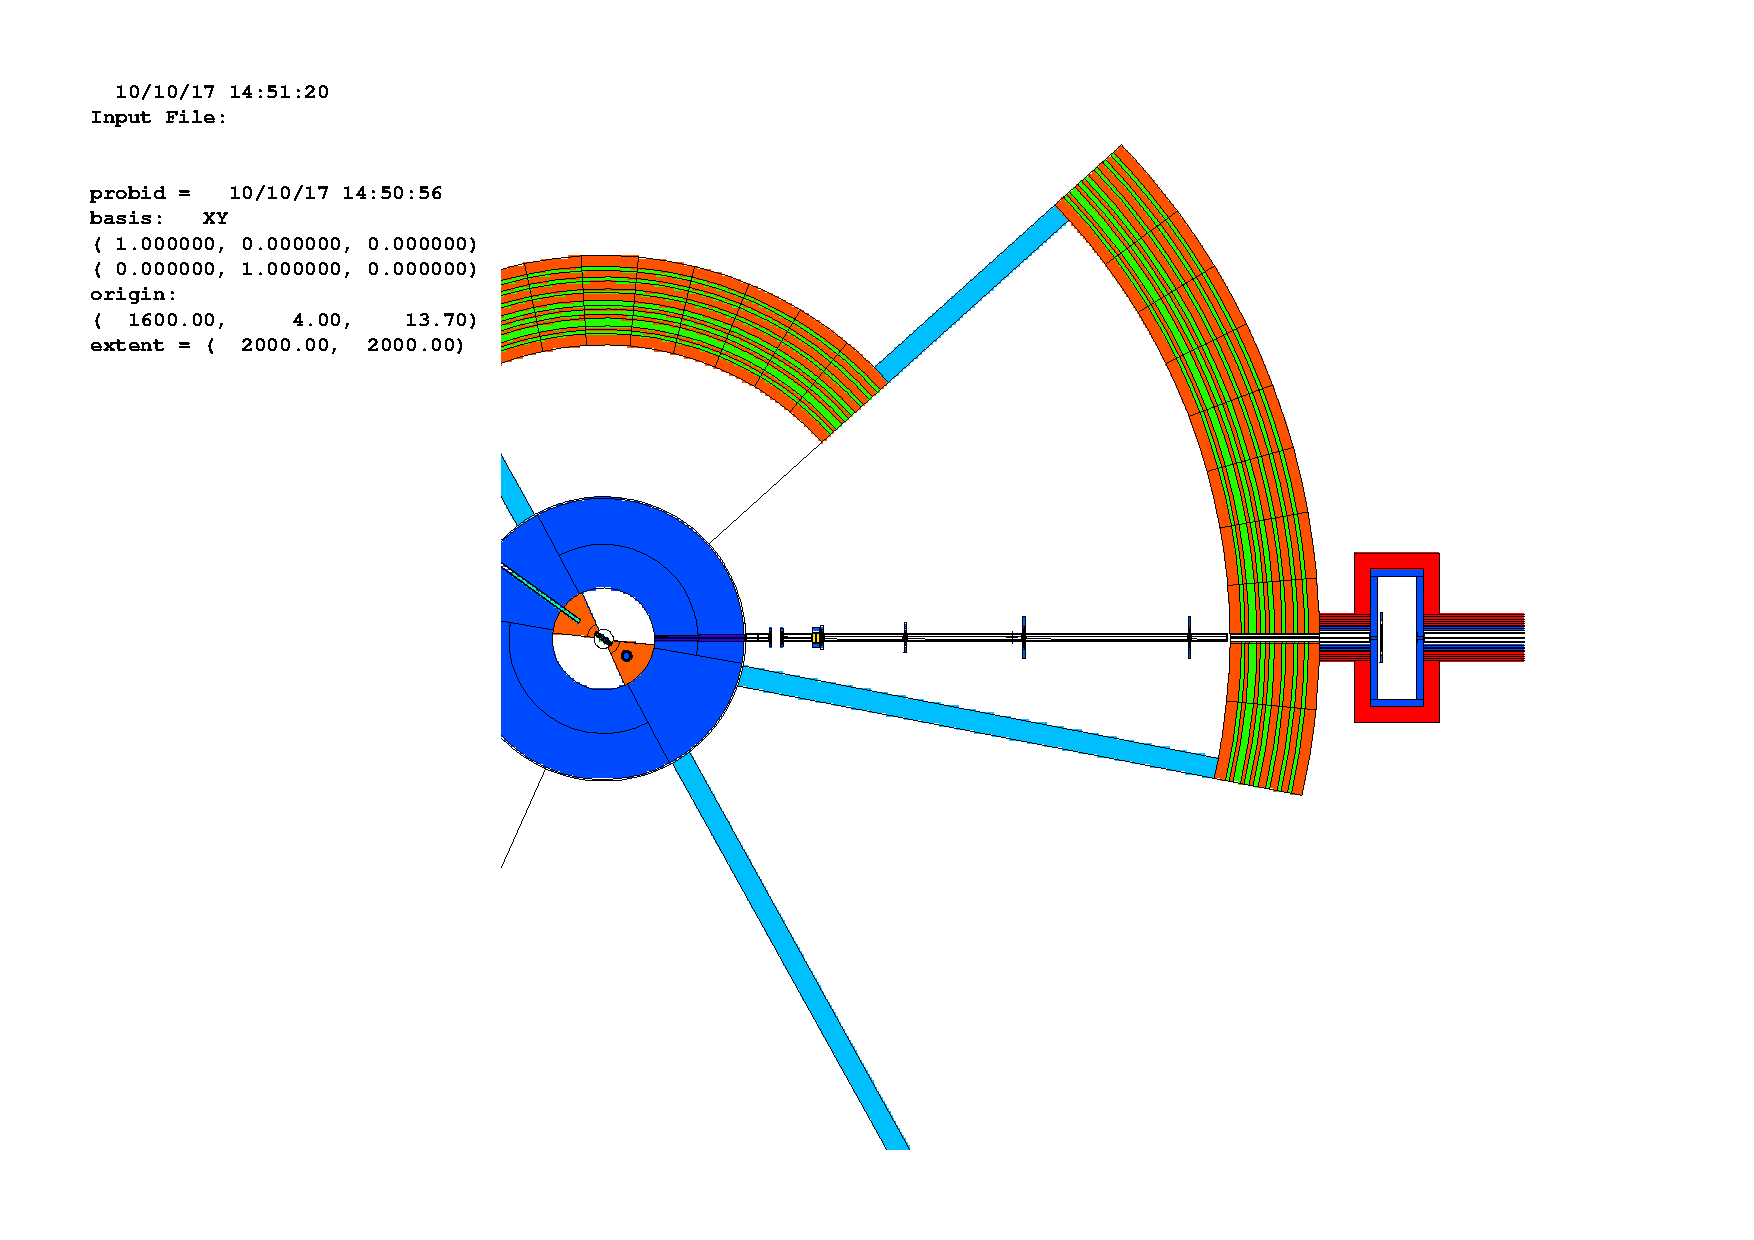
\includegraphics[width=0.5\linewidth,page=1,clip=true, trim=10cm 8cm 4cm 7cm]{UserGuide/cell-biasing.pdf}};
    \begin{scope}[x={(image.south east)},y={(image.north west)}]
      % \draw[help lines, xstep=.1, ystep=.1] (0,0) grid (1,1);
      % \foreach \x in {0,1,...,9} {\node [anchor=north] at (\x/10, 0) {0.\x}; }
      % \foreach \y in {0,1,...,9} {\node [anchor=east]  at (0, \y/10) {0.\y}; }

      \draw[red,thick] (0.07, 0.367) circle (0.5mm);
      \draw[arrow] (0.11,0.46) -- (0.077,0.38);
      \node[legend, anchor=west] at (0.1,0.5) {weightSource};

      \draw[red,dashed] (0.79,0) -- (0.79,1);
      \draw[arrow] (0.85,0.8) -- (0.79,0.8);
      \node[legend, anchor=west] at (0.85,0.8) {weightPlane};

      \draw[arrow]     (0.14,0.2) -- (0.14,0.36);
      \node[legend] at (0.14,0.2) {G2BLineTop20};

      \draw[arrow]                 (0.65,0.25) -- (0.69,0.25);
      \node[legend,anchor=east] at (0.65,0.25) {CBunkerWallMainWall1};

      \draw[arrow]                 (0.65,0.45) -- (0.69,0.45);
      \node[legend,anchor=east] at (0.65,0.45) {CBunkerWallMainWall2};
    \end{scope}
  \end{tikzpicture}
  }
  \subfloat[Horizontal view: wwn]{
    \includegraphics[width=0.5\linewidth,page=2,clip=true, trim=10cm 8cm 4cm 7cm]{UserGuide/cell-biasing.pdf}
  } \\
  \subfloat[Vertical view: geometry]{
    \includegraphics[width=0.5\linewidth,page=3,clip=true, trim=10cm 8cm 4cm 7cm]{UserGuide/cell-biasing.pdf}
  }
  \subfloat[Vertical view: wwn]{
    \includegraphics[width=0.5\linewidth,page=4,clip=true, trim=10cm 8cm 4cm 7cm]{UserGuide/cell-biasing.pdf}
  }
  \caption{Cell-based weight window}
  \label{fig:vr:cell}
\end{figure}
\end{landscape}
